\subsection{Ordnungsrelationen}\index{Ordnungsrelationen}

\begin{tabular}{c|l}
  \hline
  $a=b$                   & Gleichheit                      \\
  $\pi\ne 3$              & Ungleichheit                    \\
  $\pi\approx \frac{22}7$ & ungefähr gleich                 \\
  $a<b$                   & $a$ ist kleiner als $b$         \\
  $3>1$                   & Analog:  ... ist größer als ... \\

  $a\leq b$               & $a$ kleiner als oder gleich $b$ \\
  $a\geq 4$               & Analog: $a$ ist 4 oder größer.  \\
  \hline
\end{tabular}


\subsubsection{Intervall-Notation}

\renewcommand{\arraystretch}3
\begin{tabular}{c|c|c}

  Relation & Zahlenstrahl & Intervallschreibweise \\
  \hline
  $a \geq 4$  &
  \TRAINER{\raisebox{-5mm}{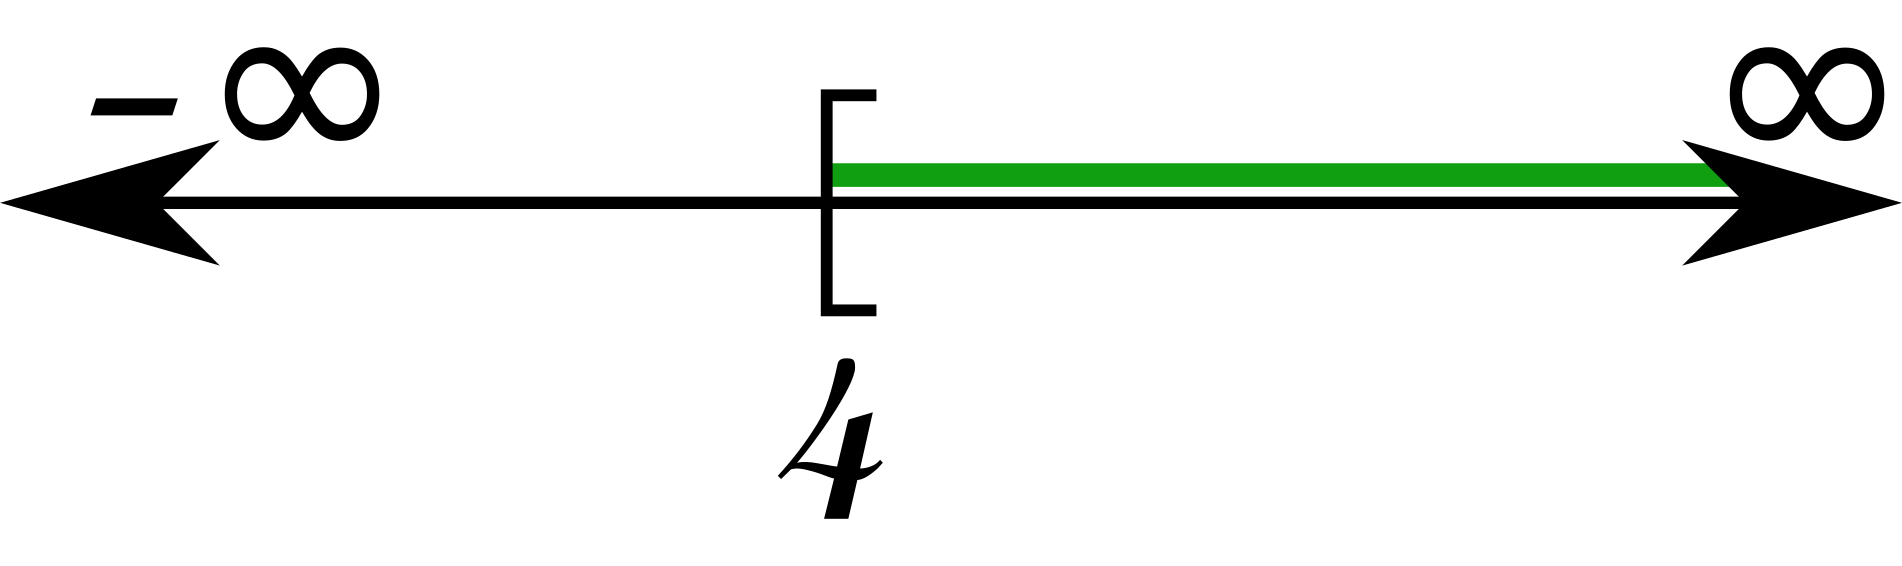
\includegraphics[width=40mm]{allg/alg/img/intervallGE4.png}}}
  \noTRAINER{\hspace{6cm}} & $[4;  \infty [$\\
      \hline
      
  $x\leq 5$ und $x > -2$  &
      \TRAINER{\raisebox{-5mm}{
\includegraphics[width=40mm]{allg/alg/img/intervallM2T5.png}}}
      & $]-2; 5]$\\
  
  \hline
  $-42 > z$  &
  \TRAINER{\raisebox{-5mm}{
\includegraphics[width=40mm]{allg/alg/img/intervallLE-42.png}}} & $] -\infty ; -42[ $\\
\hline  
\end{tabular}
\renewcommand{\arraystretch}1


\subsection*{Aufgaben zu Ordnungsrelationen}
\GESOAadB{22f}{10. b) 11. a) b) c) d)}
\TALSAadB{8-10}{\*}
\TRAINER{Spätestens hier auf die Musterlösungswege im OLAT hinweisen.}
\newpage
